\chapteropener{Data Observability}{minthard}{mintaccent}{%
Data observability monitors help check whether data arrives on time and whether its structure and values meet expectations. This chapter covers row counts, timestamps, schema changes, missing and repeated values, and summaries of numeric and text columns.

The figures follow one simulated orders table over six weeks. Rows arriving on the same day form a daily partition. Most monitors compare each day's measurement with a range learned from earlier days; schema monitoring compares column names and types directly. Gray bands show expected ranges, red points mark alerts, and hollow points indicate skipped or unavailable measurements. Each page explains one monitor, what it can detect, and what it can miss.}{In this chapter}

% ---------- Decision map ----------
\begin{decisionmap}{minthard}{mintaccent}{Which monitor?}{Follow the branches to a monitor. The number next to it is its page.}
\maproot{What could have gone wrong upstream?}
\begin{forest} dmap
[, coordinate, l sep=0pt
  [{\dl{you first want to know how any monitor decides}{\mref{Expected Range}{sec:expected-range}}}]
  [{\dm{the data is late or partial}{What do you check?}}
    [{\dl{when it last landed}{\mref{Freshness}{sec:freshness}}}]
    [{\dl{how many rows came}{\mref{Row Count}{sec:row-count}}}]
  ]
  [{\dl{the structure changed}{\mref{Schema Changes}{sec:schema-changes}}}]
  [{\dm{values are missing or repeated}{Which?}}
    [{\dl{empty cells}{\mref{Missing Values}{sec:missing-values}}}]
    [{\dl{rows that should be unique}{\mref{Duplicates}{sec:duplicates}}}]
    [{\dl{the number of distinct values}{\mref{Unique Count}{sec:unique-count}}}]
  ]
  [{\dm{numbers drifted or spiked}{Which part of the distribution?}}
    [{\dl{the center}{\mref{Average}{sec:average}}}]
    [{\dl{the total}{\mref{Sum}{sec:sum}}}]
    [{\dl{the spread}{\mref{Standard Deviation}{sec:standard-deviation}}}]
    [{\dl{the extremes}{\mref{Min and Max}{sec:min-and-max}}}]
    [{\dl{the shape}{\mref{Quartiles}{sec:quartiles}}}]
  ]
  [{\dl{text changed shape}{\mref{Text Length}{sec:text-length}}}]
]
\end{forest}
\mapnotes{Check freshness and row count alongside value monitors: incomplete loads can affect their results. Compare schema changes with the previous or approved schema.}
\end{decisionmap}

% All figures in this chapter come from one simulated `orders` table, monitored daily for 42 days
% (notebooks/observability_plots.py). Metric definitions follow the Soda documentation:
% https://docs.soda.io/data-observability/metric-monitoring-dashboard

% Wording review references:
% https://www.itl.nist.gov/div898/handbook/pmc/section3/pmc31.htm
% https://www.postgresql.org/docs/current/functions-aggregate.html
% https://numpy.org/doc/stable/reference/generated/numpy.quantile.html
% Duplicate percentage counts all non-null rows in repeated-key groups here.
% Tool conventions differ; the expected-range detector is illustrative.

% ---------- Expected Range ----------
\clearpage
\thispagestyle{observabilitystyle}
\section{Expected Range}\label{sec:expected-range}
\subsection{Comparing a Metric with Its History}

An expected range describes the values a monitor considers normal, based on earlier measurements. A value outside this range is flagged for review. In the rule below, $\mu_t$ is the expected value for the day and $\sigma_t$ describes the usual variation around it.

% equation
\begin{center}
    \tikz{
        \node[inner sep=2pt, font=\Large] (a) {
            {
                $\displaystyle
                \text{anomaly at } t \iff \big|\, {\color{nmlcyan}x_t} - {\color{nmlpurple}\mu_t} \,\big| > {\color{nmlyellow}z}\, {\color{nmlpurple}\sigma_t}
                $
            }
        };
        \draw[overlay,-latex,nmlcyan, semithick] ($(a.north)+(0.2,-0.2)$) to[bend right=15] node[pos=1, left] {today's measurement} +(-1,.5);
        \draw[overlay,-latex,nmlpurple, semithick] ($(a.north)+(1.4,-0.2)$) to[bend left=15] node[pos=1, right] {baseline from history} +(0.8,.5);
        \draw[overlay,-latex,nmlyellow, semithick] ($(a.south)+(2.0,0.25)$) to[bend right=15] node[pos=1, left] {sensitivity} +(-0.8,-.5);
        \draw[overlay,-latex,nmlpurple, semithick] ($(a.south)+(2.75,0.25)$) to[bend left=15] node[pos=1, right] {spread of history} +(0.4,-.5);
    }
\end{center}

The setting $z$ controls the width of the range. Lower values flag smaller changes; higher values allow more variation. A common choice for this type of rule is $z=3$, but settings depend on the tool. A good monitor also accepts human feedback: marking an alert as expected can help it learn a legitimate pattern; confirming an incident can help keep bad data out of its baseline.

\begin{center}
    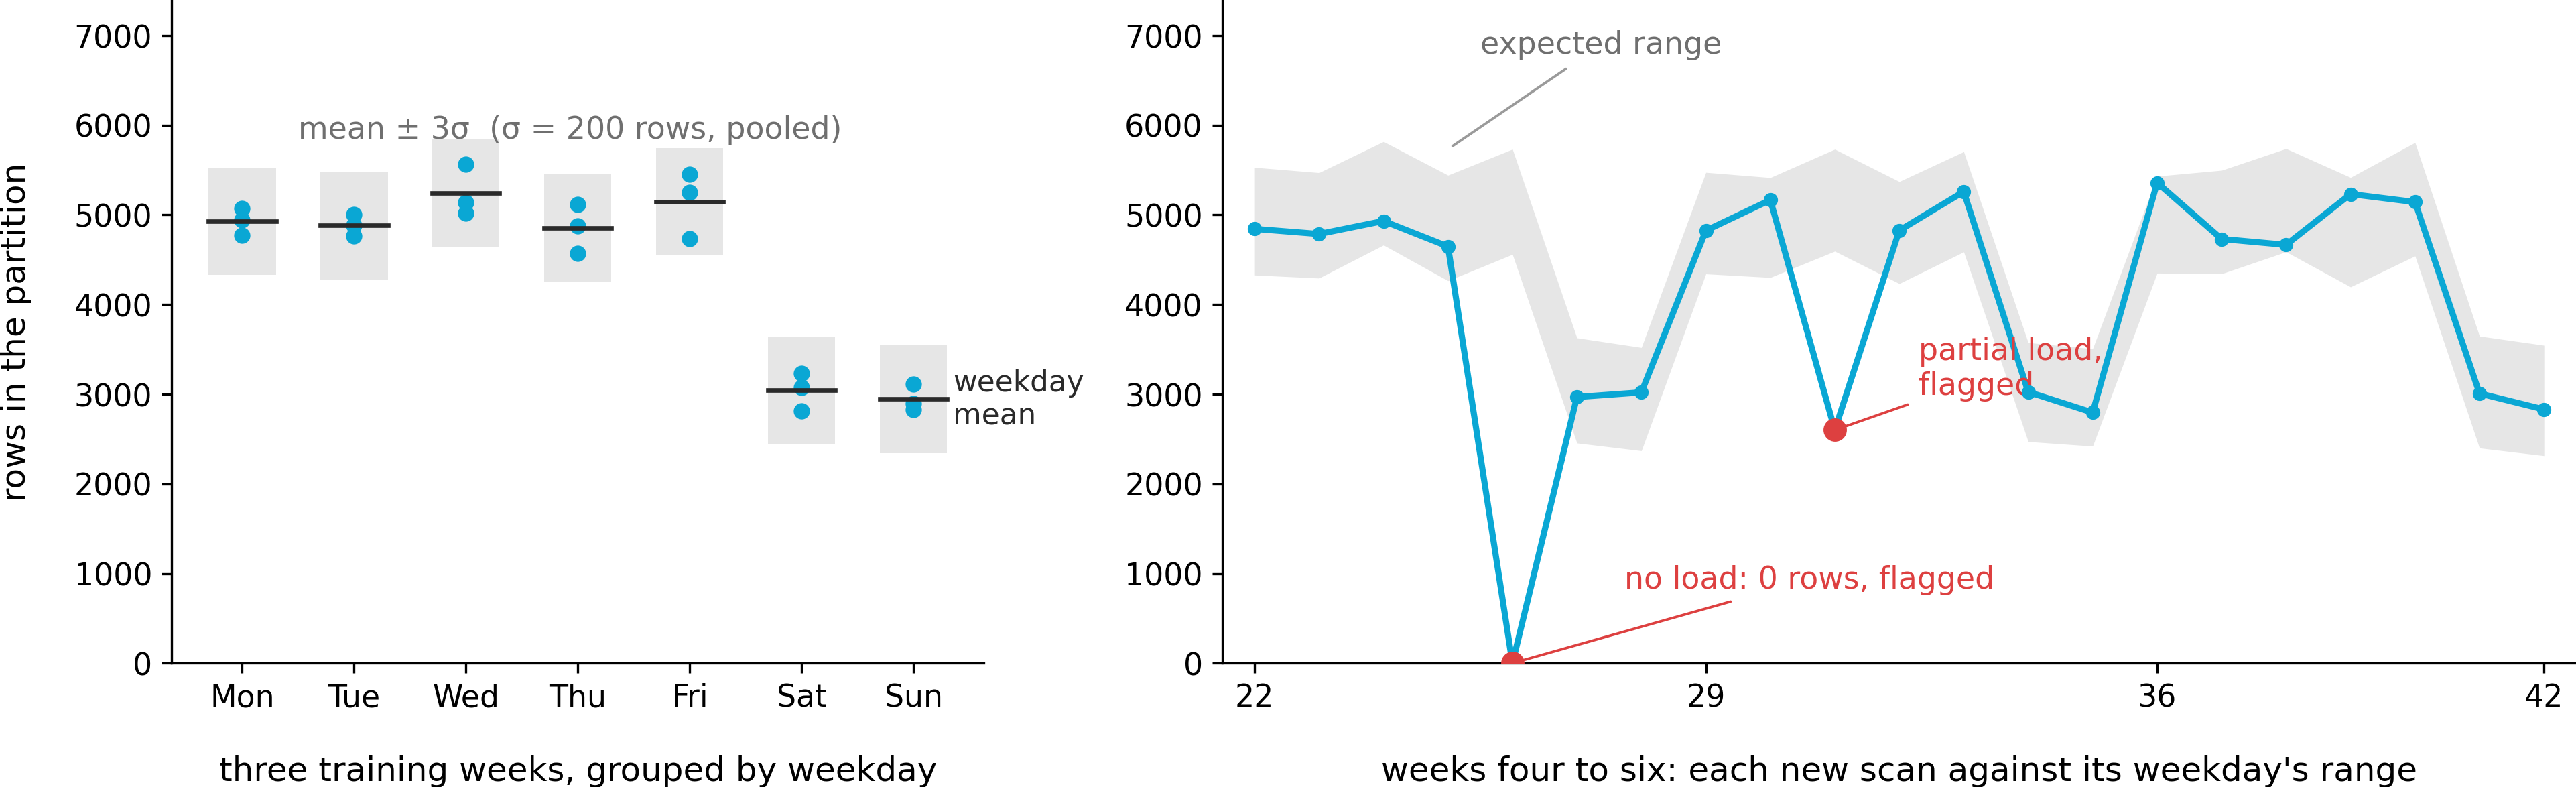
\includegraphics[width=\textwidth]{figures/Observability_expected_range.png}
\end{center}

\textbf{Figure. Expected Range.} Daily counts for a simulated orders table. \underline{Left:} three weeks of data establish an average for each weekday, with a range of about $600$ rows above and below it. \underline{Right:} no load arrives on day $26$, and only part of the load arrives on day $31$. Both counts fall below the range. Lower weekend counts stay within their expected range.

\textbf{When to use it?}

Use a historical range when normal values change over time, for example between weekdays and weekends. Adjust sensitivity to balance missed problems against false alerts. A known requirement, such as zero duplicate keys, is better checked with a fixed limit. A flagged value needs investigation; it is not necessarily an error.

% ---------- Row Count ----------
\clearpage
\thispagestyle{observabilitystyle}
\section{Row Count}\label{sec:row-count}
\subsection{Volume}

Row count tells you how many rows are in a table or a selected part of it. It helps detect missing, incomplete or repeated loads. Here, each scan counts one day's arrivals, called a daily partition.

% equation
\begin{center}
    \tikz{
        \node[inner sep=2pt, font=\Large] (a) {
            {
                $\displaystyle
                \text{rows}_{t} = \sum_{r \in T} \mathds{1}\big[\, {\color{nmlcyan}p(r)} = {\color{nmlpurple}t} \,\big]
                $
            }
        };
        \draw[overlay,-latex,nmlcyan, semithick] ($(a.south)+(0.9,0.3)$) to[bend left=15] node[pos=1, left] {row's partition value} +(-1,-.5);
        \draw[overlay,-latex,nmlpurple, semithick] ($(a.north)+(1.7,-0.2)$) to[bend left=15] node[pos=1, right] {the partition being scanned} +(0.6,.5);
    }
\end{center}

The formula counts rows whose partition date $p(r)$ matches the day $t$ being checked. In SQL, this is \texttt{COUNT(*)} with a date filter. Some databases also provide a row count in their metadata, but it may be approximate or out of date.

\begin{center}
    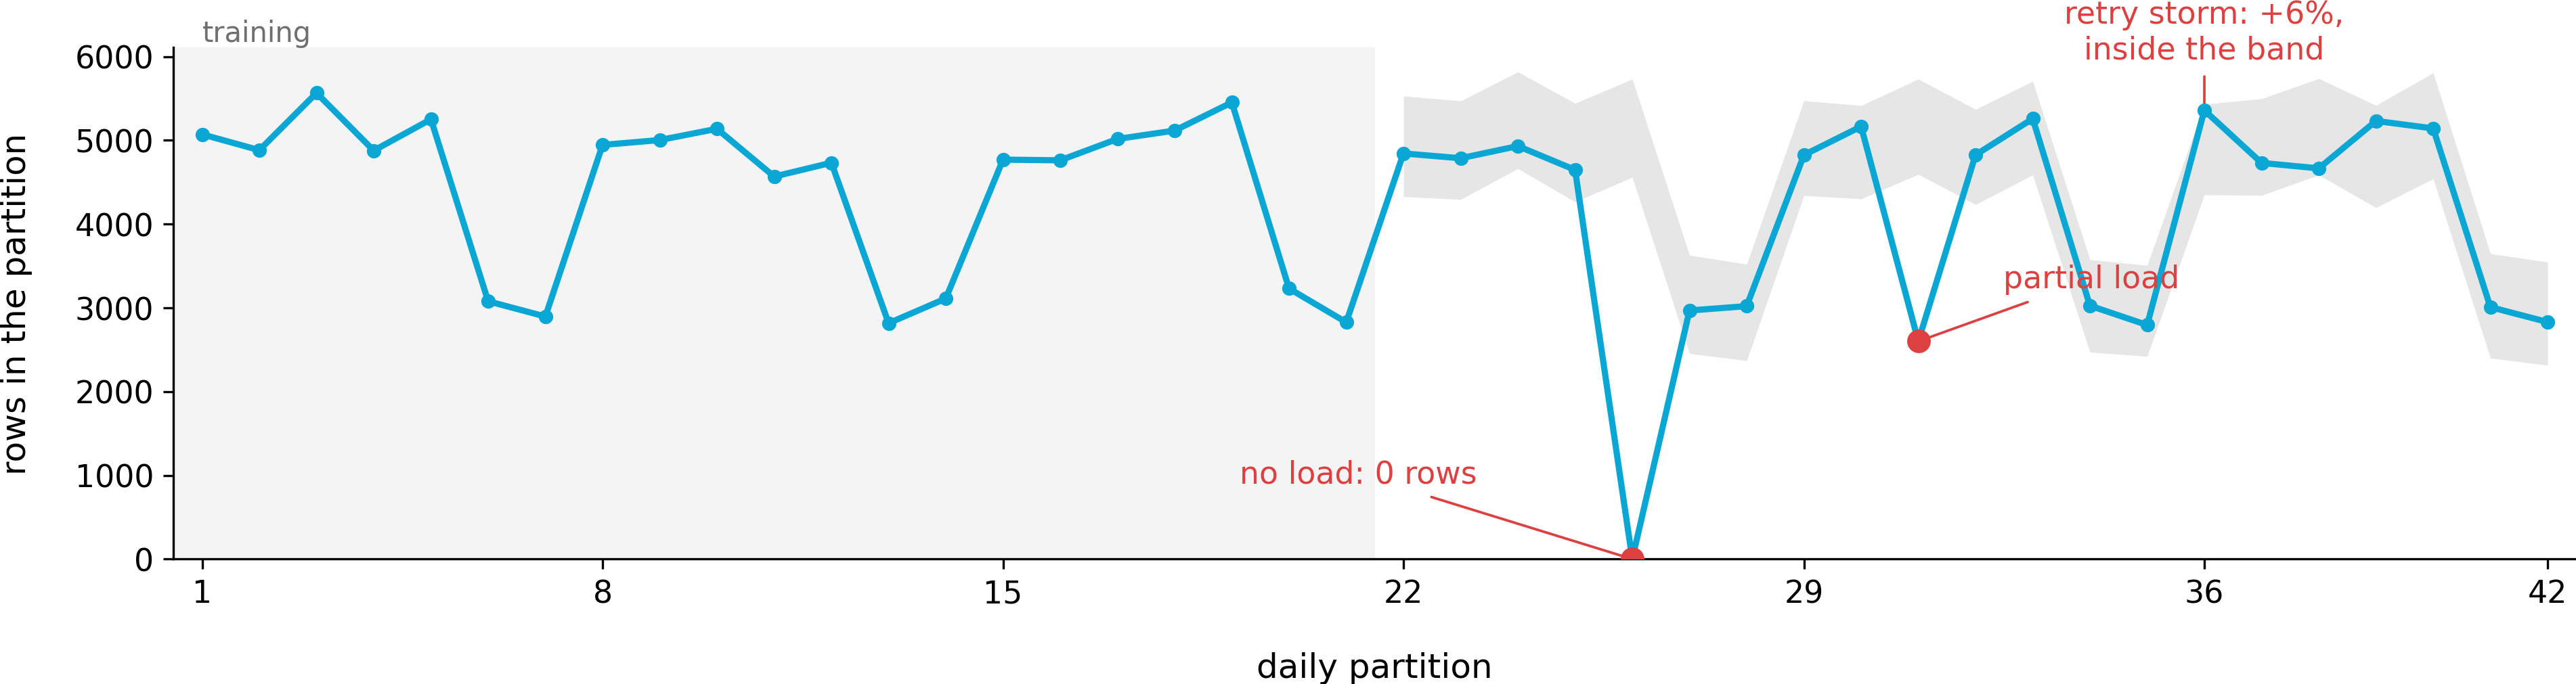
\includegraphics[width=\textwidth]{figures/Observability_row_count.png}
\end{center}

\textbf{Figure. Row Count.} Daily row counts for an orders table. Day $26$ has no rows and day $31$ has only $2{,}600$; both are below the expected range. On day $36$, some rows are loaded twice, bringing the count to $5{,}358$. That is still inside the range, so row count alone misses the repeated rows.

\textbf{When to use it?}

Use it to check whether a scheduled load delivered the expected amount of data. Compare equivalent periods and account for patterns such as quieter weekends. If rows can arrive late, recheck earlier days too. A normal count does not guarantee that the rows are correct or unique.

% ---------- Freshness ----------
\clearpage
\thispagestyle{observabilitystyle}
\section{Freshness}\label{sec:freshness}
\subsection{Most Recent Timestamp}

Freshness measures how much time has passed since the latest timestamp in a column. With an arrival timestamp, it tells you when data last reached the table. With an event timestamp, it tells you when the latest recorded event happened.

% equation
\begin{center}
    \tikz{
        \node[inner sep=2pt, font=\Large] (a) {
            {
                $\displaystyle
                \text{freshness}_t = {\color{nmlpurple}t_{\text{scan}}} - \max_{r \in T} {\color{nmlcyan}\text{ts}(r)}
                $
            }
        };
        \path[room for labels] ([yshift=0.57cm]a.north) ([yshift=-0.00cm]a.south);
        \draw[overlay,-latex,nmlpurple, semithick] ($(a.north)+(0.19,-0.09)$) to[bend right=15] node[pos=1, left] {time of the scan} +(-1.00,0.30);
        \draw[overlay,-latex,nmlcyan, semithick] ($(a.north)+(2.76,-0.03)$) to node[pos=1, above] {newest timestamp} +(0.00,0.30);
    }
\end{center}

The formula subtracts the newest timestamp from the scan time, ignoring nulls. If the latest arrival is at 01:30 and the scan is at 06:00, freshness is $4.5$ hours. Some databases also record when a table was last updated. That can be checked without reading its rows, but an update does not prove that newer data arrived.

\begin{center}
    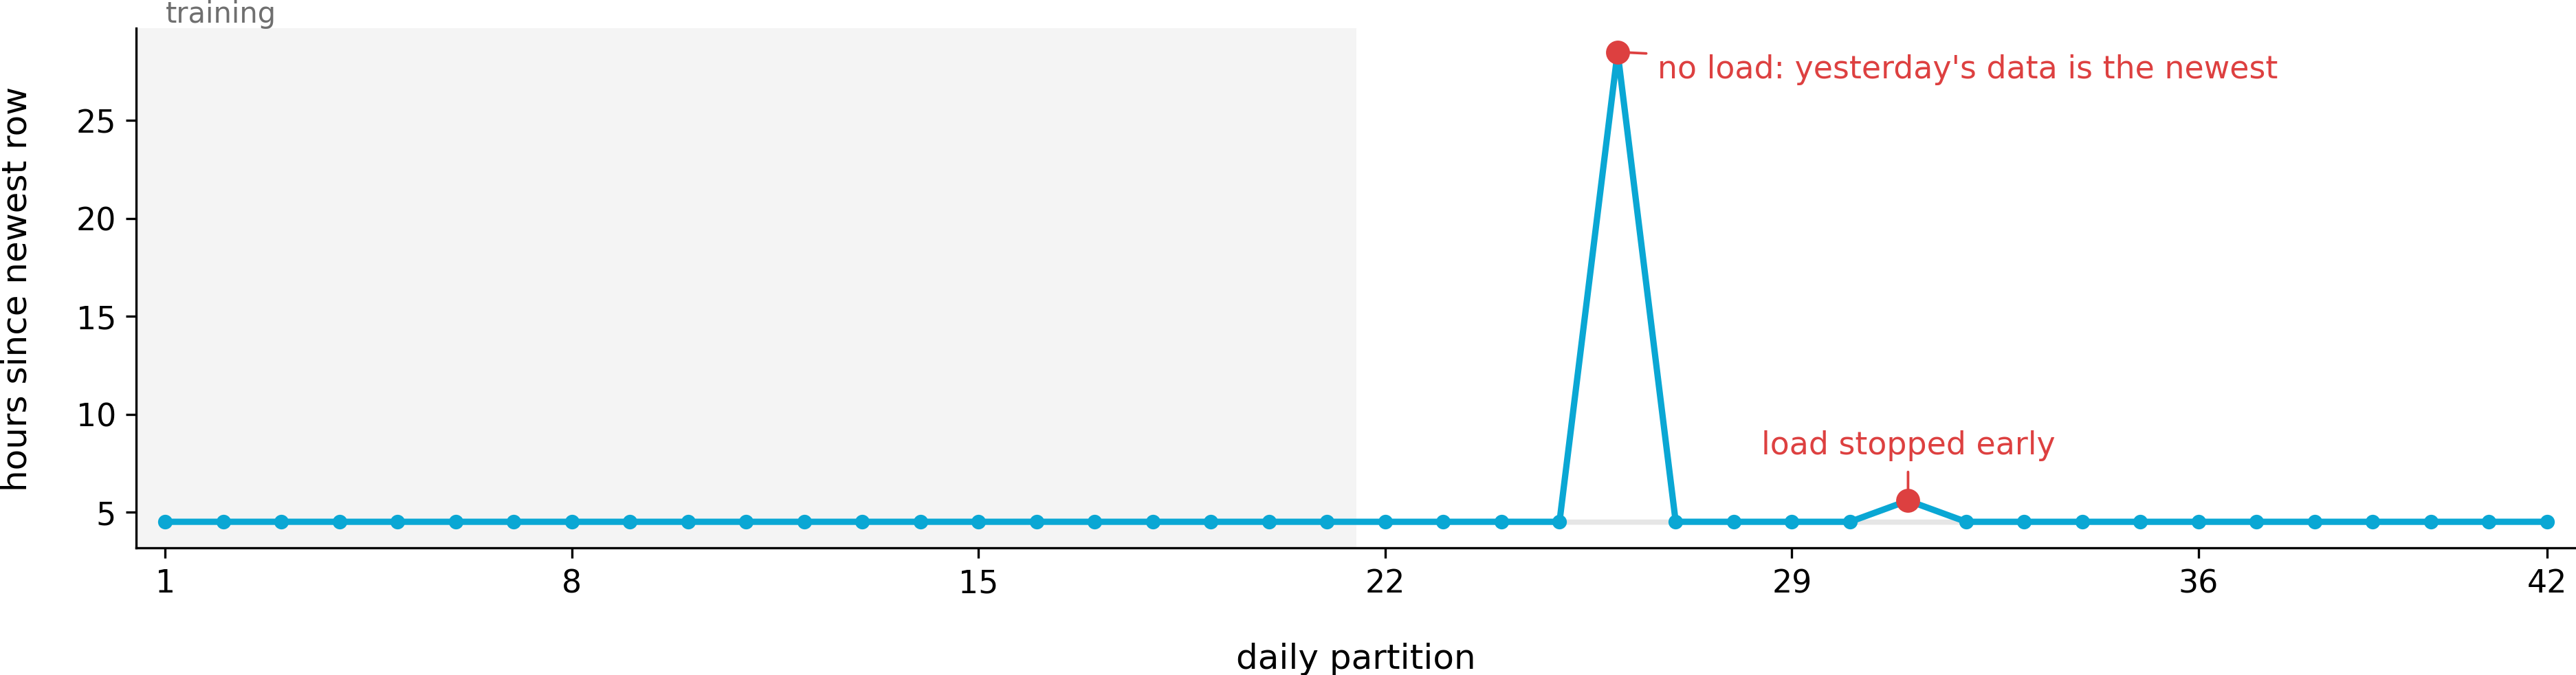
\includegraphics[width=\textwidth]{figures/Observability_freshness.png}
\end{center}

\textbf{Figure. Freshness.} The orders table is scanned at 06:00, usually $4.5$ hours after its latest arrival. Nothing arrives on day $26$, so freshness reaches $28.5$ hours. The load stops early on day $31$, leaving the newest row $5.6$ hours old. Both days are flagged.

\textbf{When to use it?}

Use it when data must arrive before a deadline. Choose the timestamp that matches what you need to check, and allow for the loading schedule and time zone. Check row count too: one recent row can make an incomplete load look fresh. Without a valid timestamp, freshness cannot be calculated.

% ---------- Schema Changes ----------
\clearpage
\thispagestyle{observabilitystyle}
\section{Schema Changes}\label{sec:schema-changes}
\subsection{Columns and Types}

Schema monitoring detects changes to column names and data types. It can tell you when a column is added, removed or given a different type. These changes may break queries or alter how values are stored, even when the data still loads successfully.

% equation
\begin{center}
    \tikz{
        \node[inner sep=2pt, font=\Large] (a) {
            {
                $\displaystyle
                \Delta_t = {\color{nmlcyan}S_t} \,\triangle\, {\color{nmlpurple}S_{t-1}}, \qquad \text{anomaly} \iff \Delta_t \neq \varnothing
                $
            }
        };
        \path[room for labels] ([yshift=0.50cm]a.north) ([yshift=-0.47cm]a.south);
        \draw[overlay,-latex,nmlcyan, semithick] ($(a.north)+(-3.34,-0.03)$) to node[pos=1, above] {columns and types now} +(0.00,0.22);
        \draw[overlay,-latex,nmlpurple, semithick] ($(a.south)+(-1.69,0.07)$) to node[pos=1, below] {at the previous scan} +(0.00,-0.22);
    }
\end{center}

Each $S$ lists the column names and types at one scan. The $\triangle$ compares two lists and keeps only the differences. A renamed column appears as one removal and one addition. The check flags changes for review; an intentional change is not necessarily a problem.

\begin{center}
    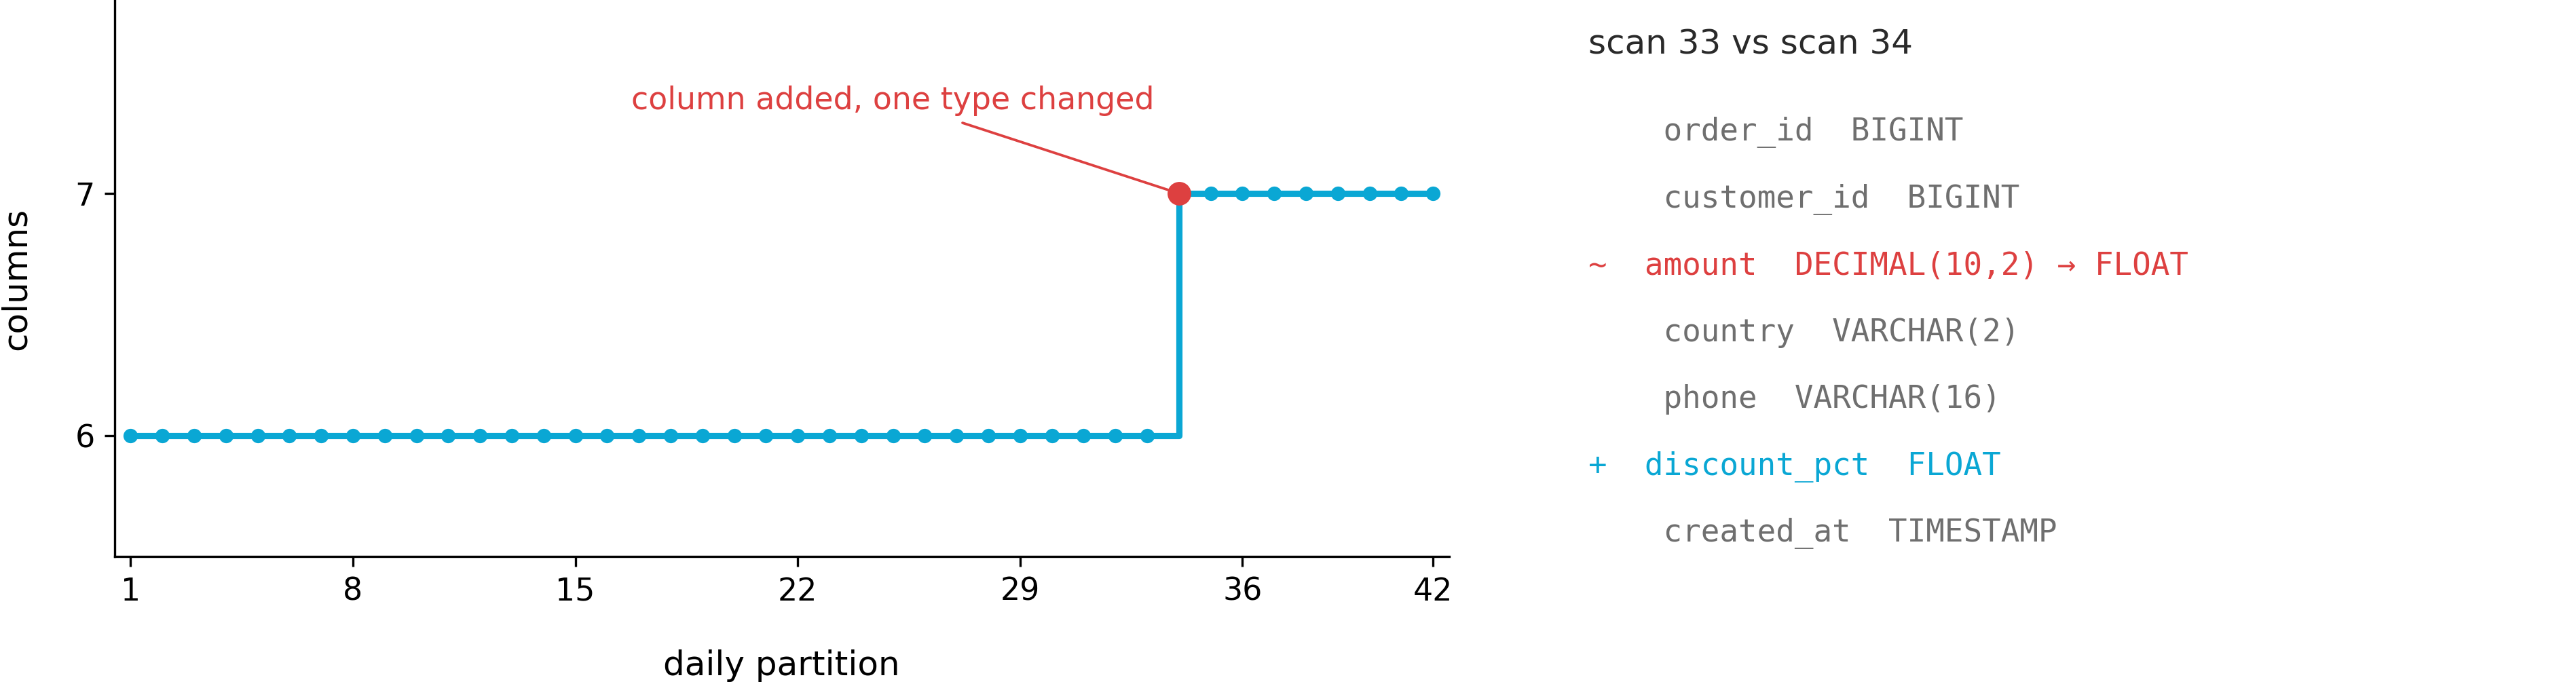
\includegraphics[width=\textwidth]{figures/Observability_schema.png}
\end{center}

\textbf{Figure. Schema Changes.} \underline{Left:} the table grows from six columns to seven on day $34$. \underline{Right:} \texttt{discount\_pct} is added and \texttt{amount} changes from \texttt{DECIMAL(10,2)} to \texttt{FLOAT}. The column count shows the addition, but only comparing the types reveals the second change.

\textbf{When to use it?}

Use it on tables that other queries, applications or models depend on. Check whether a change affects those uses before accepting it. Changes to the values themselves can go unnoticed: storing cents instead of dollars may leave the column name and type unchanged.

% ---------- Missing Values ----------
\clearpage
\thispagestyle{observabilitystyle}
\section{Missing Values}\label{sec:missing-values}
\subsection{Completeness}

Missing values percentage tells you what share of a column's values are null. It helps check whether needed information is present. For example, a rise in missing country codes may indicate that a source field is no longer being loaded correctly.

% equation
\begin{center}
    \tikz{
        \node[inner sep=2pt, font=\Large] (a) {
            {
                $\displaystyle
                \text{missing}\%_t = 100 \cdot \left( 1 - \frac{{\color{nmlcyan}\text{count}(c)}}{{\color{nmlred}\text{count}(*)}} \right)
                $
            }
        };
        \path[room for labels] ([yshift=0.24cm]a.north) ([yshift=-0.19cm]a.south);
        \draw[overlay,-latex,nmlcyan, semithick] ($(a.north)+(2.37,-0.04)$) to[bend right=15] node[pos=1, left] {non-null values in the column} +(-1.00,0.30);
        \draw[overlay,-latex,nmlred, semithick] ($(a.south)+(2.29,0.10)$) to[bend left=15] node[pos=1, left] {rows in the partition} +(-1.00,-0.30);
    }
\end{center}

The formula compares the number of filled rows, $\text{count}(c)$, with the total number of rows, $\text{count}(*)$. If $80$ of $100$ rows are filled, the missing percentage is $20\%$. This check counts nulls; blank text and placeholders such as \texttt{N/A} may need separate rules.

\begin{center}
    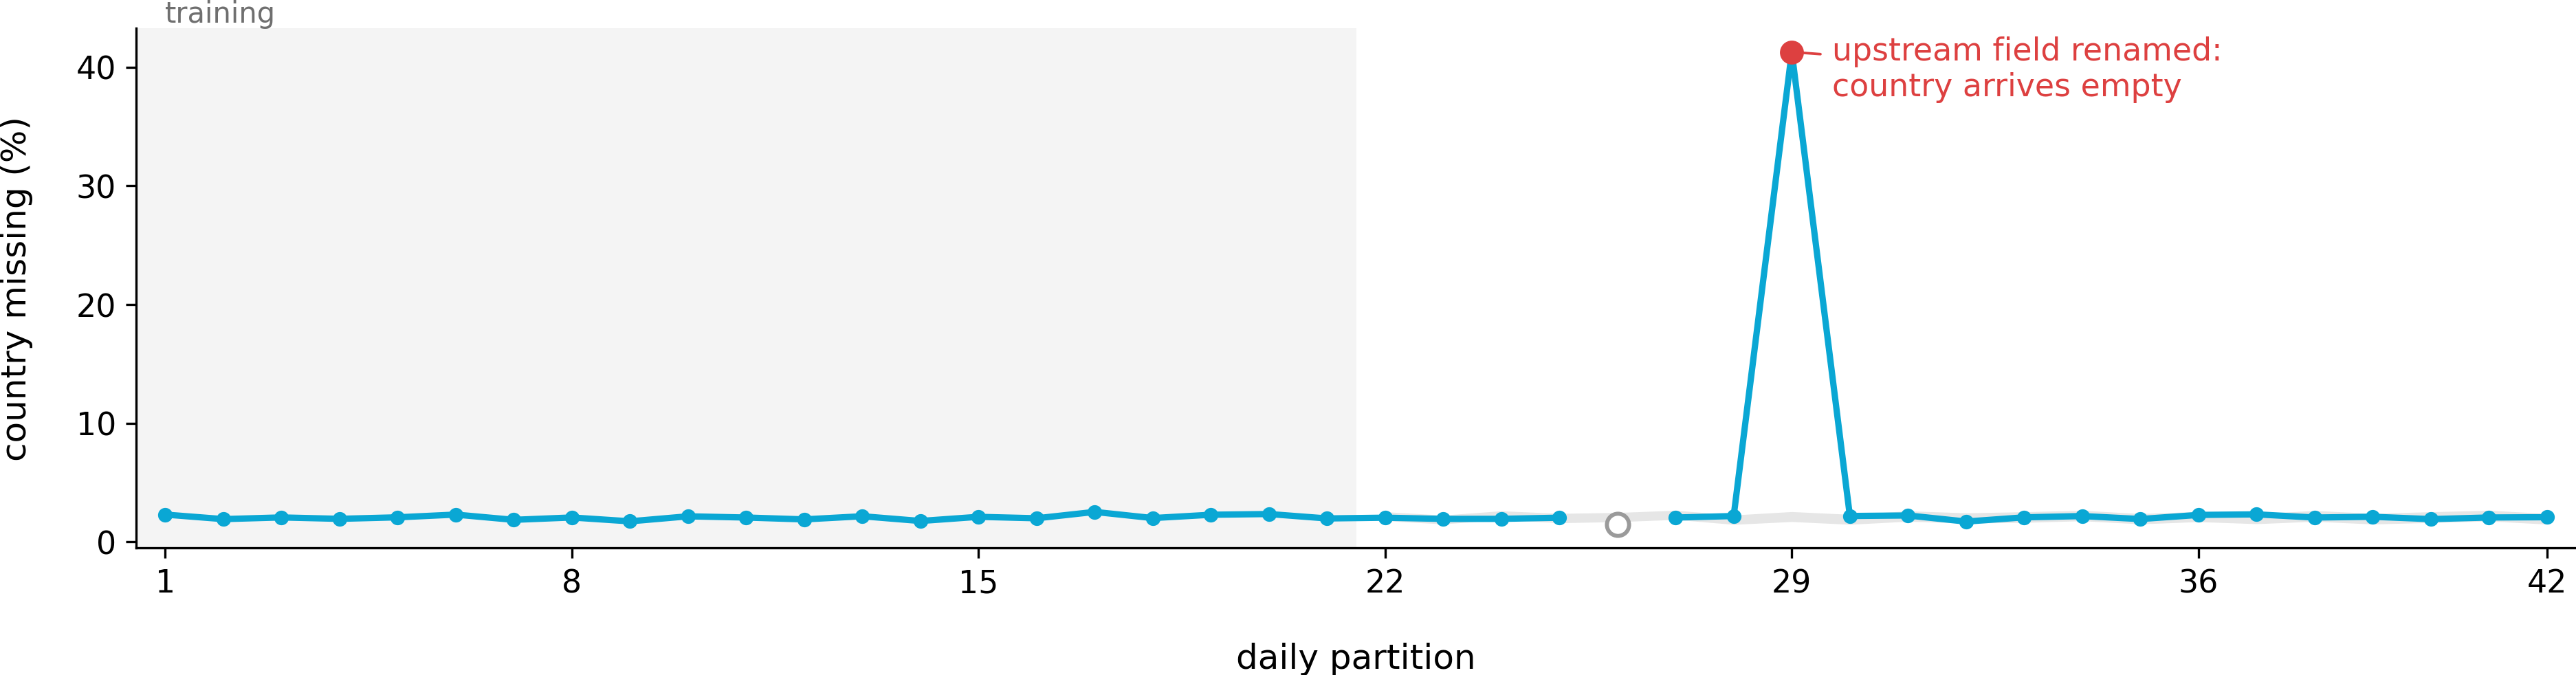
\includegraphics[width=\textwidth]{figures/Observability_missing.png}
\end{center}

\textbf{Figure. Missing Values.} About $2\%$ of country values are normally null. On day $29$, a source-field rename leaves $41\%$ missing, so the monitor flags the increase. The hollow point on day $26$ marks a day with no rows: there is no percentage to calculate.

\textbf{When to use it?}

Use it on fields needed for joins, reports or model inputs. Set the acceptable level according to the field: an optional field may legitimately contain nulls. Replacing missing values with a placeholder such as \texttt{unknown} can make the percentage fall without improving the data.

% ---------- Duplicates ----------
\clearpage
\thispagestyle{observabilitystyle}
\section{Duplicates}\label{sec:duplicates}
\subsection{Uniqueness}

Duplicate percentage shows what share of rows have a repeated key. A key is a value, such as an order ID, used to identify a record. Here, every copy counts as a duplicate, and rows with null keys are excluded.

% equation
\begin{center}
    \tikz{
        \node[inner sep=2pt, font=\Large] (a) {
            {
                $\displaystyle
                \text{dup}\%_t = 100 \cdot \frac{1}{{\color{nmlred}|R|}} \sum_{r \in R} \mathds{1}\big[\, {\color{nmlred}n(v_r)} > 1 \,\big]
                $
            }
        };
        \draw[overlay,-latex,nmlred, semithick] ($(a.south)+(-0.29,0.25)$) to node[pos=1, below] {records with a non-null value} +(0.00,-0.30);
        \draw[overlay,-latex,nmlred, semithick] ($(a.north)+(2.10,-0.33)$) to node[pos=1, above] {how often record $r$'s value occurs} +(0.00,0.33);
    }
\end{center}

The set $R$ contains rows with a key, and $n(v_r)$ counts how often each key appears. For keys $[101,101,205,\text{null},\text{null}]$, three rows have a key and two share $101$. The duplicate percentage is therefore $2/3 \approx 66.7\%$. Some tools count only the extra copies, so check their definition.

\begin{center}
    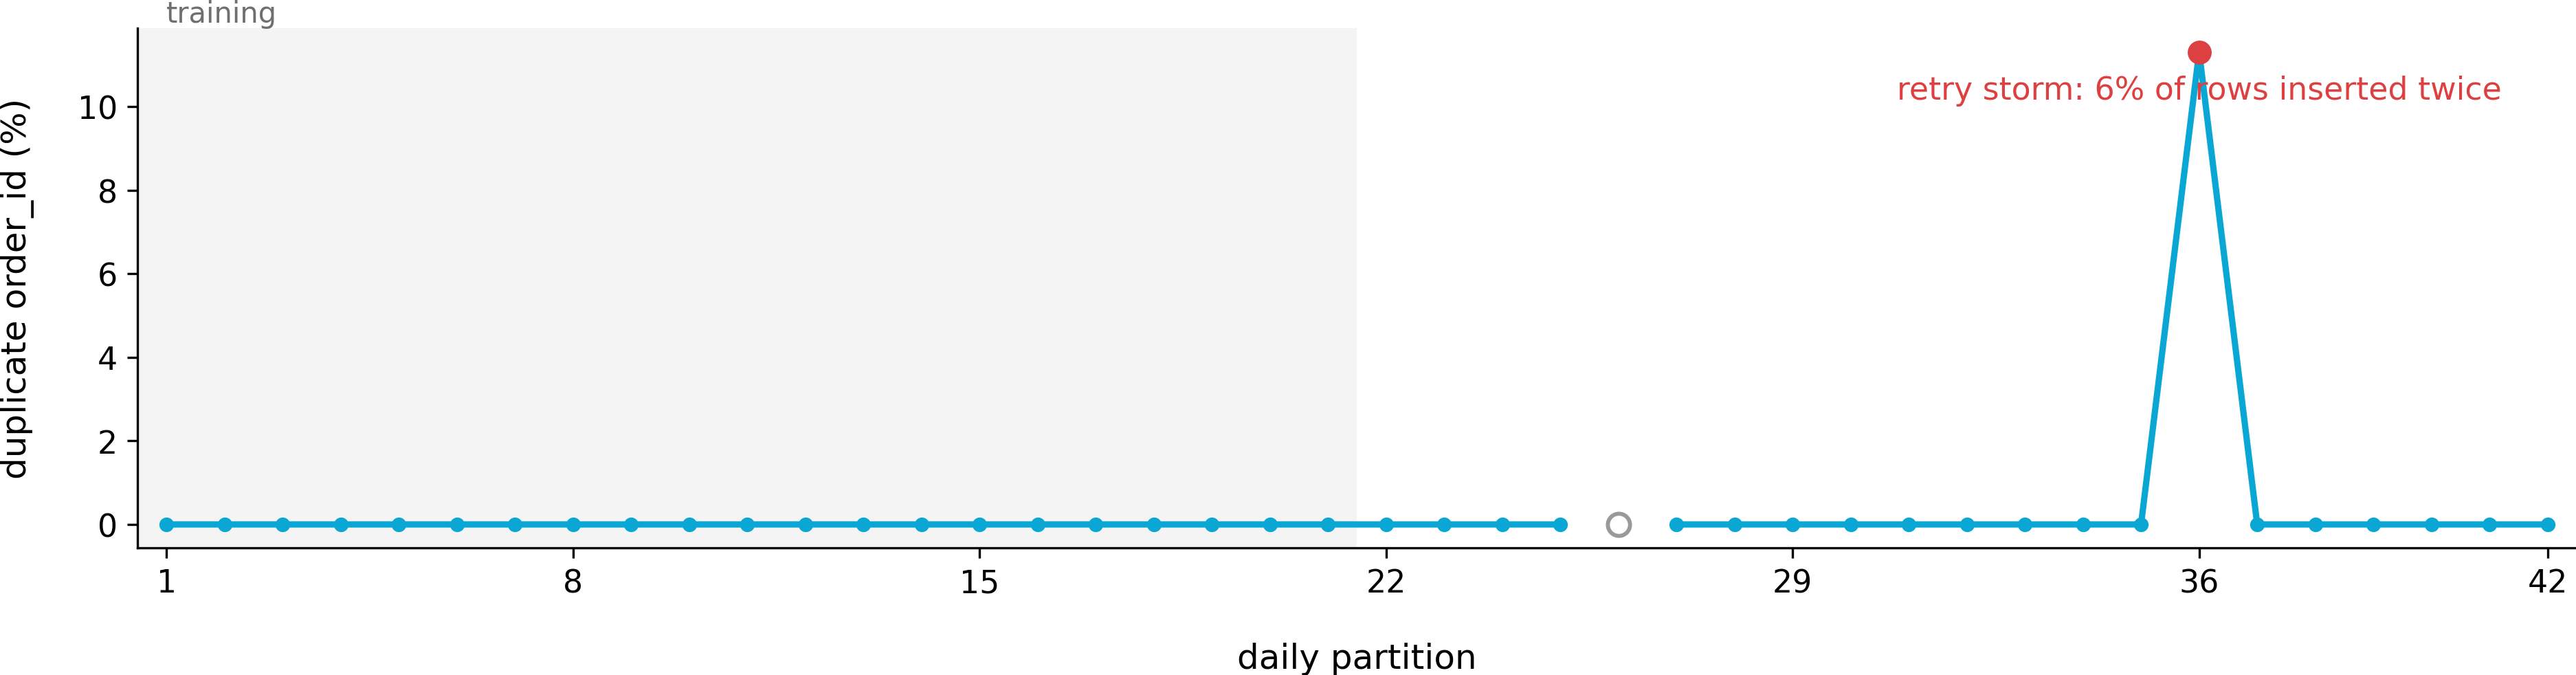
\includegraphics[width=\textwidth]{figures/Observability_duplicates.png}
\end{center}

\textbf{Figure. Duplicates.} Order IDs are unique except on day $36$, when $6\%$ of a load is inserted twice. For every $100$ original rows, six extra copies bring the total to $106$. The six originals and their copies make $12$ rows with repeated IDs: about $11.3\%$. The monitor flags this increase.

\textbf{When to use it?}

Use it on fields, or combinations of fields, that should identify rows uniquely. If any duplicate is an error, use a fixed limit of zero. Check missing keys separately. If keys must be unique across the whole table, checking only the latest day's rows is not enough.

% ---------- Unique Count ----------
\clearpage
\thispagestyle{observabilitystyle}
\section{Unique Count}\label{sec:unique-count}
\subsection{Cardinality}

Unique count tells you how many different values appear in a column. Each value counts once, even if it appears in many rows. Nulls are excluded. In an orders table, counting unique customer IDs tells you how many different customers placed an order.

% equation
\begin{center}
    \tikz{
        \node[inner sep=2pt, font=\Large] (a) {
            {
                $\displaystyle
                \text{unique}_t = \big|\, \{\, {\color{nmlcyan}c(r)} : r \in P_t,\; c(r) \neq \text{null} \,\} \,\big|
                $
            }
        };
        \path[room for labels] ([yshift=0.55cm]a.north) ([yshift=-0.00cm]a.south);
        \draw[overlay,-latex,nmlcyan, semithick] ($(a.north)+(-1.02,-0.09)$) to node[pos=1, above] {value of the column in row $r$} +(0.00,0.33);
    }
\end{center}

Here, $P_t$ is the group of rows being checked and $c(r)$ is the value in each row. For example, customer IDs $[101,101,205,\text{null}]$ give a unique count of $2$: only $101$ and $205$ are counted.

\begin{center}
    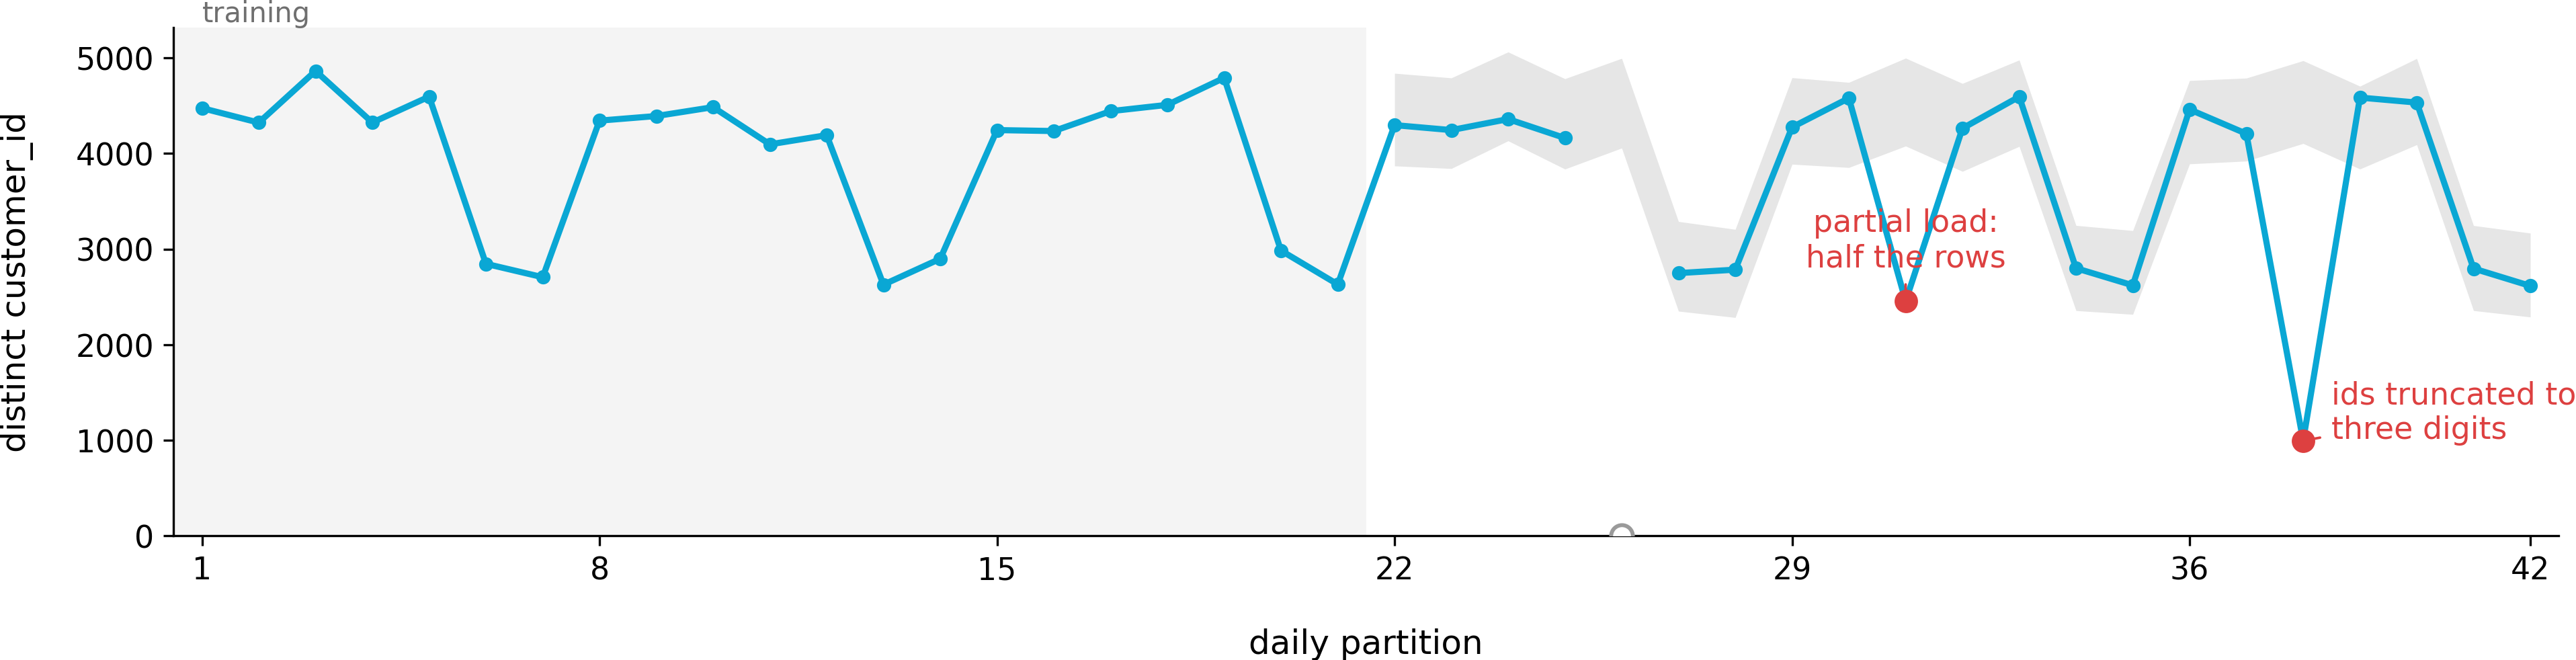
\includegraphics[width=\textwidth]{figures/Observability_unique_count.png}
\end{center}

\textbf{Figure. Unique Count.} Daily counts of different customer IDs. Weekends normally have fewer customers than weekdays. On day $31$, an incomplete load reduces the count. On day $38$, IDs are shortened to their last three digits, so different IDs become identical. Only $995$ unique values remain despite a normal load size. The hollow point marks day $26$, when no rows arrived and the check was skipped.

\textbf{When to use it?}

Use it to monitor customer IDs, product codes or categories such as countries. If unique count falls, check whether fewer rows arrived before investigating the values. It counts different values but does not tell you what they are: replacing one country code with another can leave the count unchanged.

% ---------- Average ----------
\clearpage
\thispagestyle{observabilitystyle}
\section{Average}\label{sec:average}
\subsection{Mean}

The average, or mean, is the sum of a column's values divided by how many values there are. Nulls are left out. Tracking the average can reveal a change in prices, quantities or other numeric data even when the row count stays the same.

% equation
\begin{center}
    \tikz{
        \node[inner sep=2pt, font=\Large] (a) {
            {
                $\displaystyle
                \bar{x}_t = \frac{1}{{\color{nmlred}n_t}} \sum_{r \in P_t} {\color{nmlcyan}x(r)}
                $
            }
        };
        \draw[overlay,-latex,nmlred, semithick] ($(a.south)+(-0.40,0.33)$) to node[pos=1, below] {non-null values in the partition} +(0.00,-0.30);
        \draw[overlay,-latex,nmlcyan, semithick] ($(a.north)+(1.30,-0.33)$) to[bend right=15] node[pos=1, left] {numeric value in row $r$} +(-1.00,0.61);
    }
\end{center}

Here, $n_t$ counts the values used in the calculation. For $[10,20,30]$, the average is $20$. A few very large values can raise it sharply. Increases and decreases can also cancel out, so the same average can describe very different data.

\begin{center}
    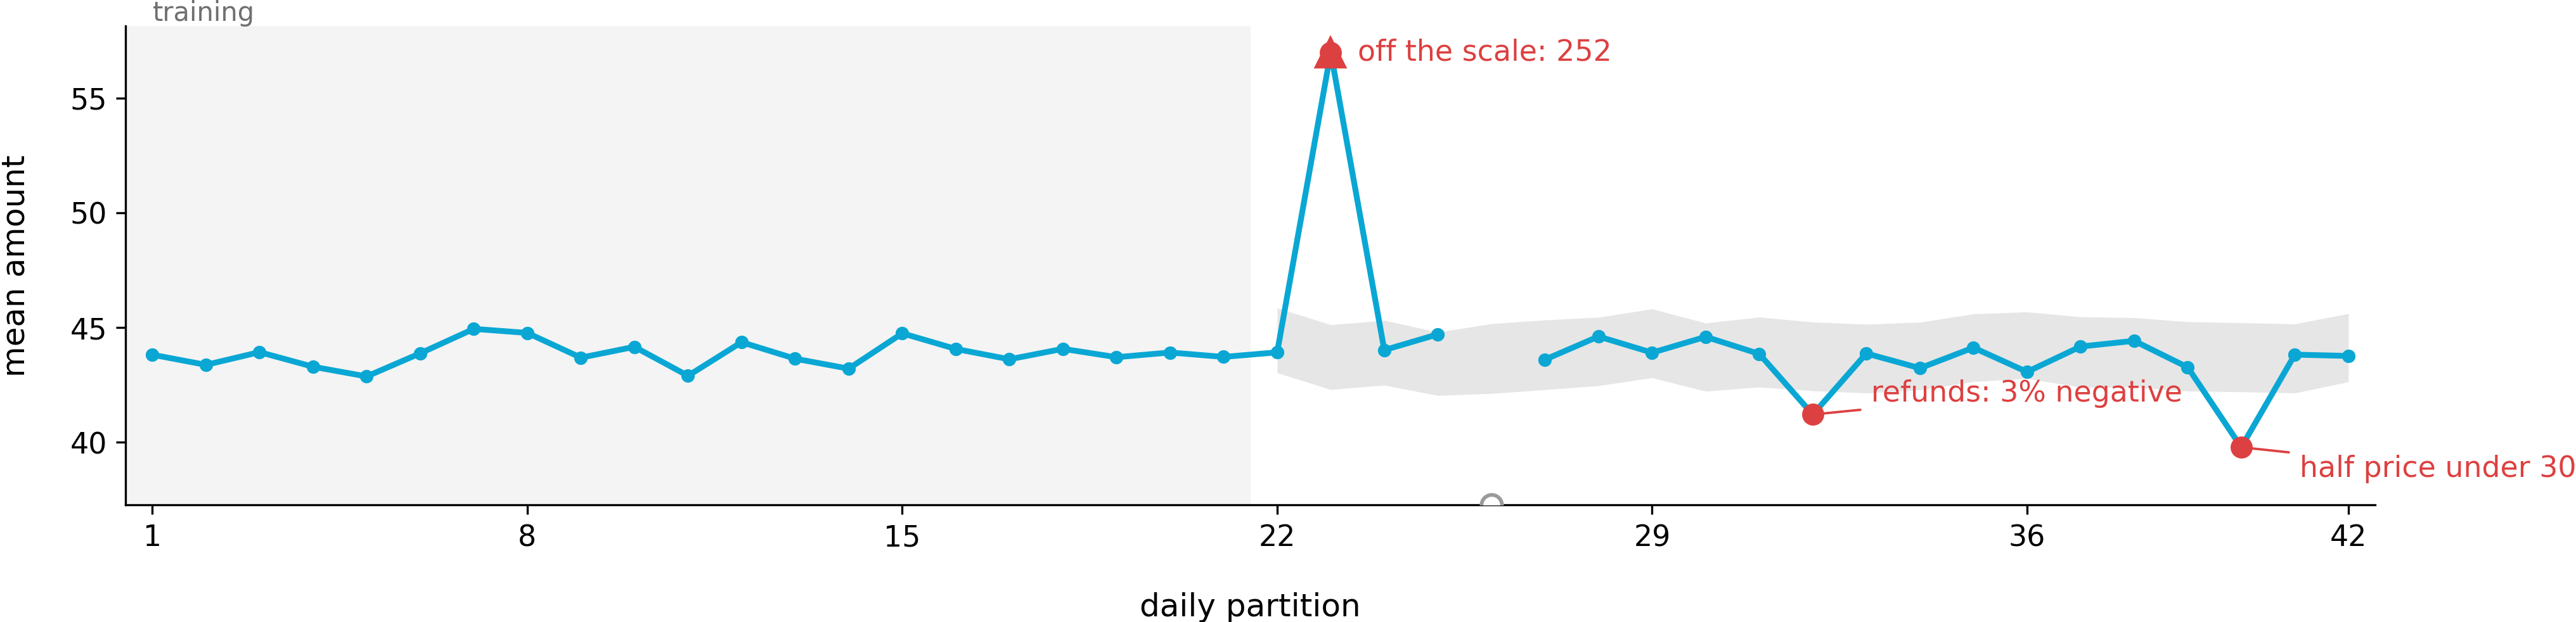
\includegraphics[width=\textwidth]{figures/Observability_average.png}
\end{center}

\textbf{Figure. Average.} Daily mean order amount. On day $23$, about $5\%$ of amounts arrive in cents instead of currency units. The mean rises from about $44$ to $252$, above the plotted scale. Negative refunds on day $32$ and discounts on amounts below $30$ on day $40$ lower the mean. All three changes are flagged.

\textbf{When to use it?}

Use it to track the overall level of a numeric column. Check quartiles and spread to understand what changed. The median is less affected by a few extreme values. A change in the average can also be legitimate, for example during a promotion.

% ---------- Sum ----------
\clearpage
\thispagestyle{observabilitystyle}
\section{Sum}\label{sec:sum}
\subsection{Total}

The sum adds up the values in a numeric column, ignoring nulls. It can track daily revenue or total units sold. A total can change because more rows arrived, because the values changed, or both.

% equation
\begin{center}
    \tikz{
        \node[inner sep=2pt, font=\Large] (a) {
            {
                $\displaystyle
                \Sigma_t = \sum_{r \in P_t} {\color{nmlcyan}x(r)} = {\color{nmlred}n_t} \cdot {\color{nmlpurple}\bar{x}_t}
                $
            }
        };
        \draw[overlay,-latex,nmlcyan, semithick] ($(a.north)+(-0.2,-0.2)$) to[bend right=15] node[pos=1, left] {numeric value in row $r$} +(-0.8,.5);
        \draw[overlay,-latex,nmlred, semithick] ($(a.south)+(1.4,0.3)$) to[bend left=15] node[pos=1, left] {rows} +(-0.4,-.5);
        \draw[overlay,-latex,nmlpurple, semithick] ($(a.north)+(2.2,-0.2)$) to[bend left=15] node[pos=1, right] {mean} +(0.6,.5);
    }
\end{center}

The sum also equals the number of non-null values $n_t$ times their average $\bar{x}_t$. For $[10,20,30]$, the total is $60$: three values with an average of $20$. SQL \texttt{SUM} returns null when there are no values to add.

\begin{center}
    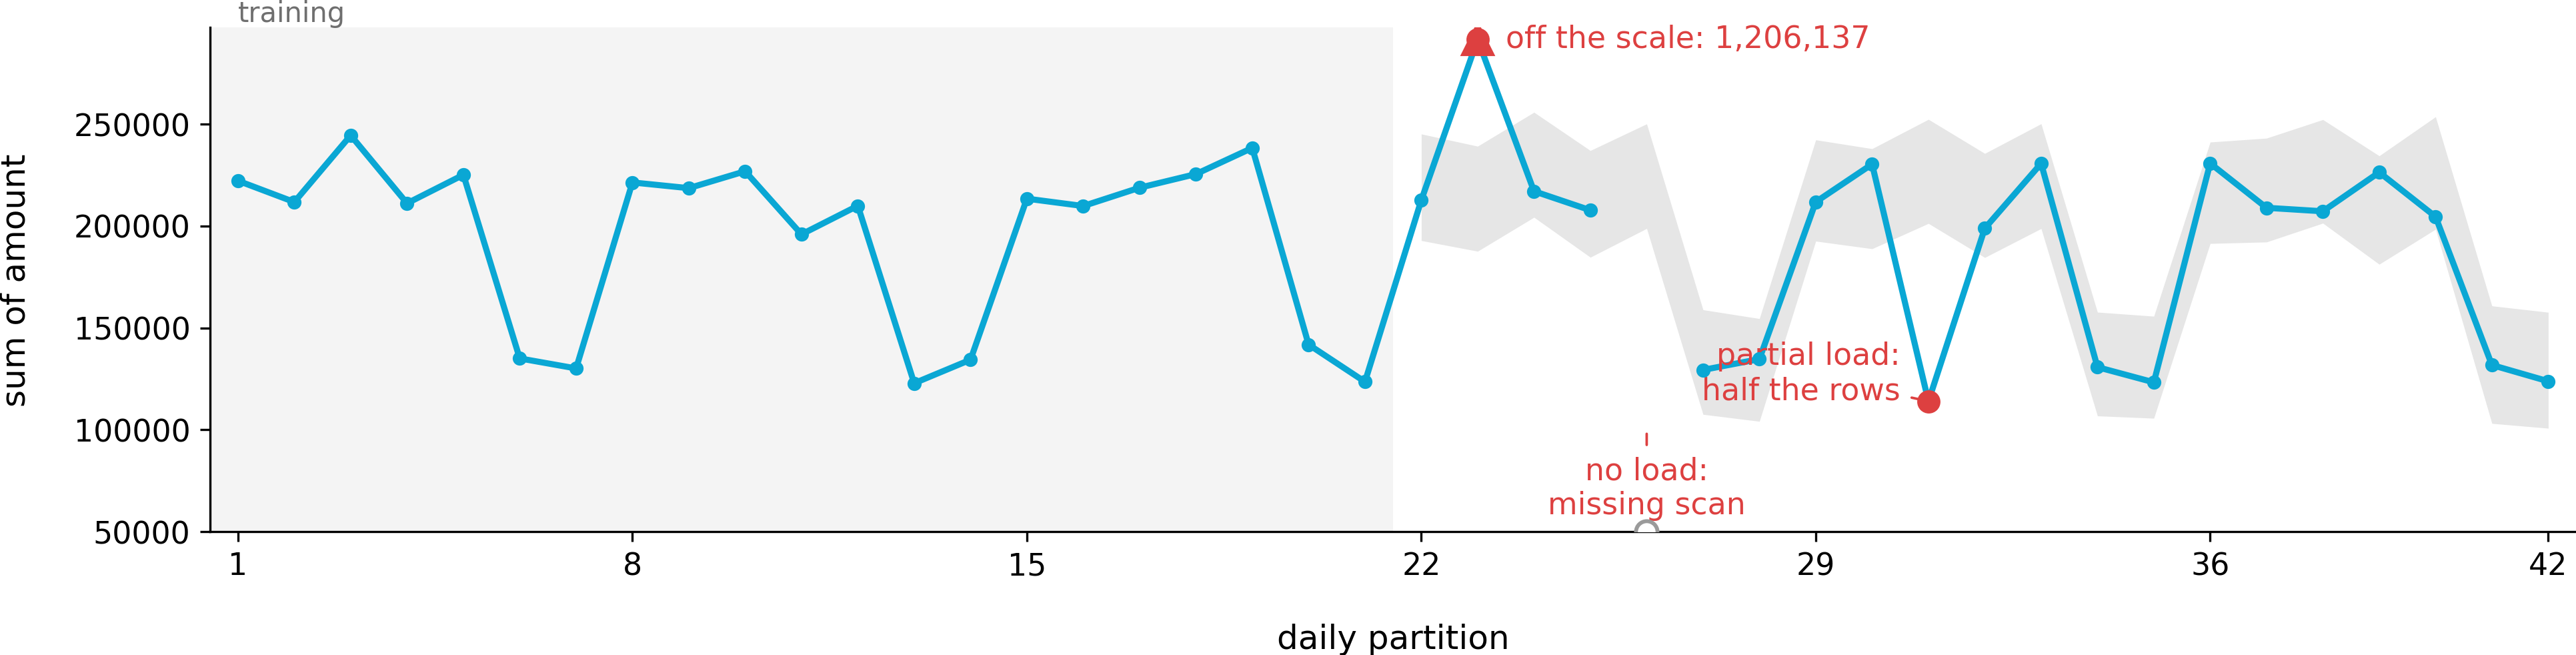
\includegraphics[width=\textwidth]{figures/Observability_sum.png}
\end{center}

\textbf{Figure. Sum.} Daily total order amount. On day $23$, about $5\%$ of amounts are stored in cents, making the total roughly six times larger. The incomplete load on day $31$ roughly halves it. Discounts on day $40$ do not push the total outside its expected range: daily changes in volume make this smaller change harder to detect.

\textbf{When to use it?}

Use it when a report depends on a total. To investigate an alert, check the number of filled rows and their average. A normal total can hide a problem if fewer rows contain larger values, or more rows contain smaller ones.

% ---------- Standard Deviation ----------
\clearpage
\thispagestyle{observabilitystyle}
\section{Standard Deviation}\label{sec:standard-deviation}
\subsection{Spread}

Standard deviation measures how much numeric values vary around their average. A larger value means they are more spread out; zero means they are all the same. It is expressed in the same units as the original values.

% equation
\begin{center}
    \tikz{
        \node[inner sep=2pt, font=\Large] (a) {
            {
                $\displaystyle
                s_t = \sqrt{ \frac{1}{{\color{nmlred}n_t} - 1} \sum_{r \in P_t} \big( {\color{nmlcyan}x(r)} - {\color{nmlpurple}\bar{x}_t} \big)^2 }
                $
            }
        };
        \draw[overlay,-latex,nmlred, semithick] ($(a.south)+(-0.9,0.3)$) to[bend left=15] node[pos=1, left] {non-null values} +(-0.6,-.5);
        \draw[overlay,-latex,nmlcyan, semithick] ($(a.north)+(1.0,-0.2)$) to[bend right=15] node[pos=1, left] {value in row $r$} +(-0.8,.5);
        \draw[overlay,-latex,nmlpurple, semithick] ($(a.north)+(2.3,-0.2)$) to[bend left=15] node[pos=1, right] {partition mean} +(0.6,.5);
    }
\end{center}

For example, $[20,20,20]$ and $[10,20,30]$ both average $20$, but only the second set has any spread. The formula gives the sample standard deviation and needs at least two non-null values. Some tools use the population version, which divides by $n_t$ rather than $n_t-1$.

\begin{center}
    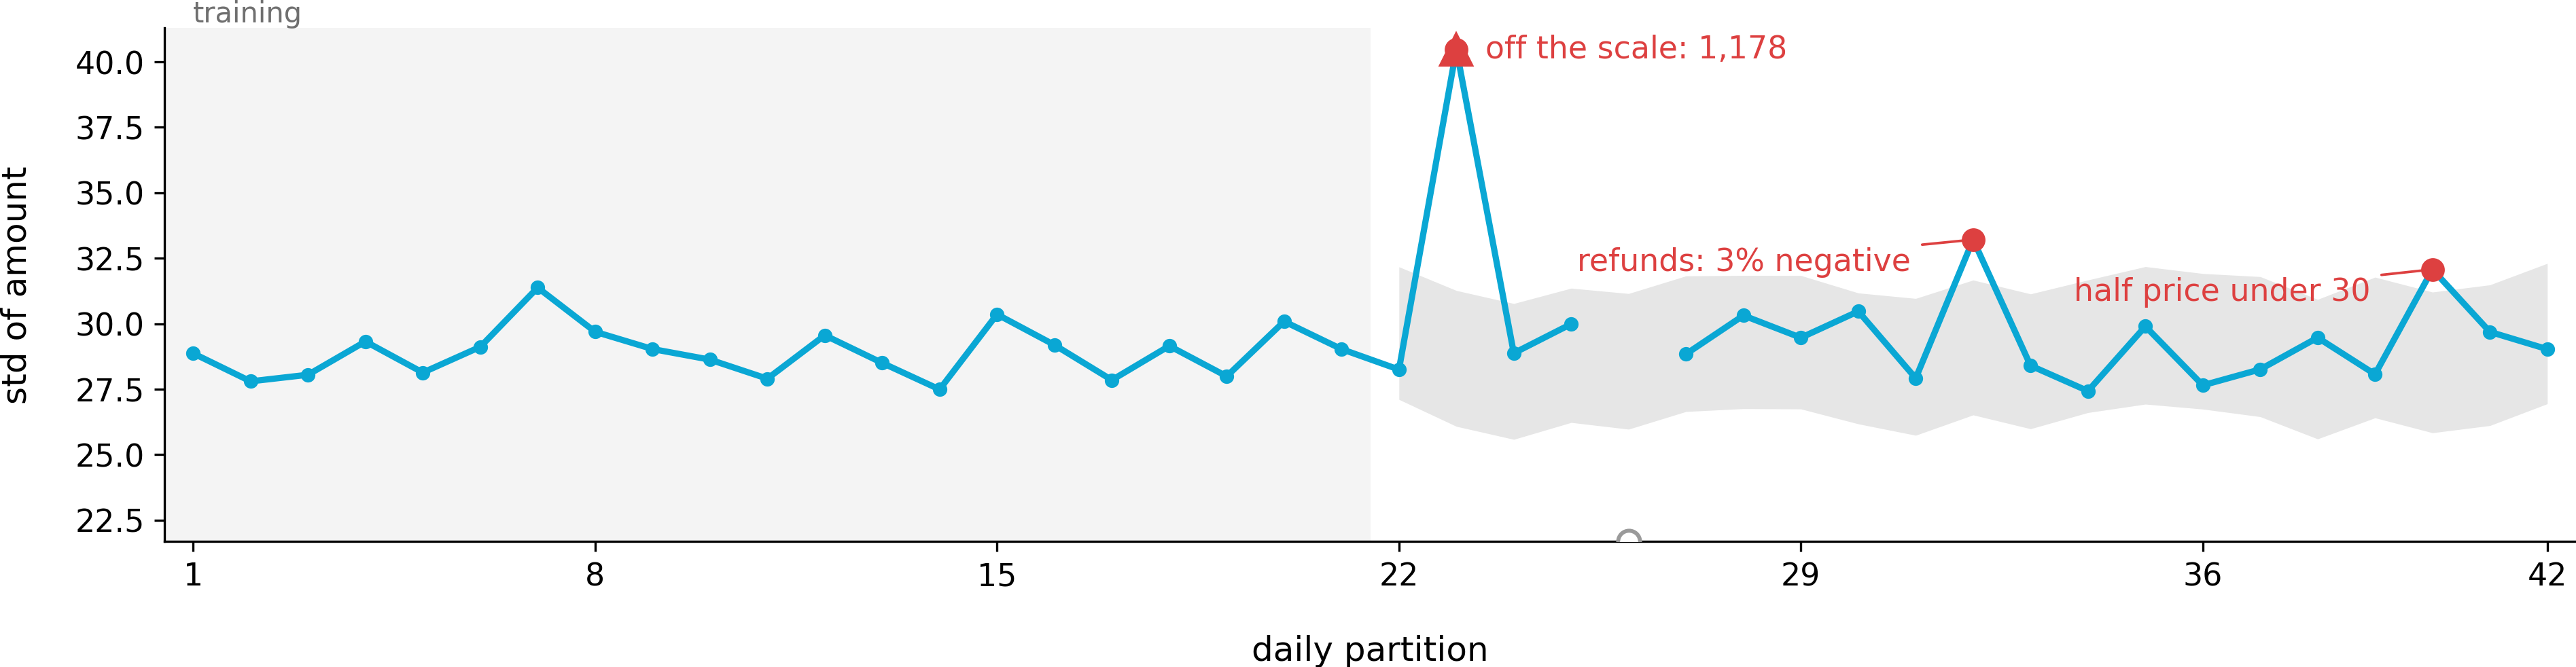
\includegraphics[width=\textwidth]{figures/Observability_stddev.png}
\end{center}

\textbf{Figure. Standard Deviation.} Daily spread of order amounts. On day $23$, about $5\%$ of amounts arrive in cents, increasing the spread about fortyfold, above the plotted scale. Negative refunds on day $32$ and discounts on amounts below $30$ on day $40$ also increase the spread. All three days are flagged.

\textbf{When to use it?}

Use it alongside the average to check how widely values vary. A few extreme values can strongly affect it, so inspect them before treating an alert as an error. Quartiles are less affected by those extremes and help show whether most values have changed.

% ---------- Min / Max ----------
\clearpage
\thispagestyle{observabilitystyle}
\section{Min and Max}\label{sec:min-and-max}
\subsection{Range}

Minimum and maximum are the smallest and largest values in a column, ignoring nulls. They help detect extreme values that an average can hide. For example, a single negative quantity changes the minimum even if thousands of other quantities are valid.

% equation
\begin{center}
    \tikz{
        \node[inner sep=2pt, font=\Large] (a) {
            {
                $\displaystyle
                \min_t = \min_{r \in P_t} {\color{nmlcyan}x(r)}, \qquad \max_t = \max_{r \in P_t} {\color{nmlpurple}x(r)}
                $
            }
        };
        \draw[overlay,-latex,nmlcyan, semithick] ($(a.north)+(-1.17,-0.04)$) to node[pos=1, above] {smallest non-null value} +(0.00,0.30);
        \draw[overlay,-latex,nmlpurple, semithick] ($(a.north)+(3.74,-0.04)$) to node[pos=1, above] {largest non-null value} +(0.00,0.30);
    }
\end{center}

The formula takes both values from the rows in $P_t$, the partition being checked. Only one row determines each result. That makes these checks sensitive to individual errors, but also to legitimate extremes, such as an unusually large order.

\begin{center}
    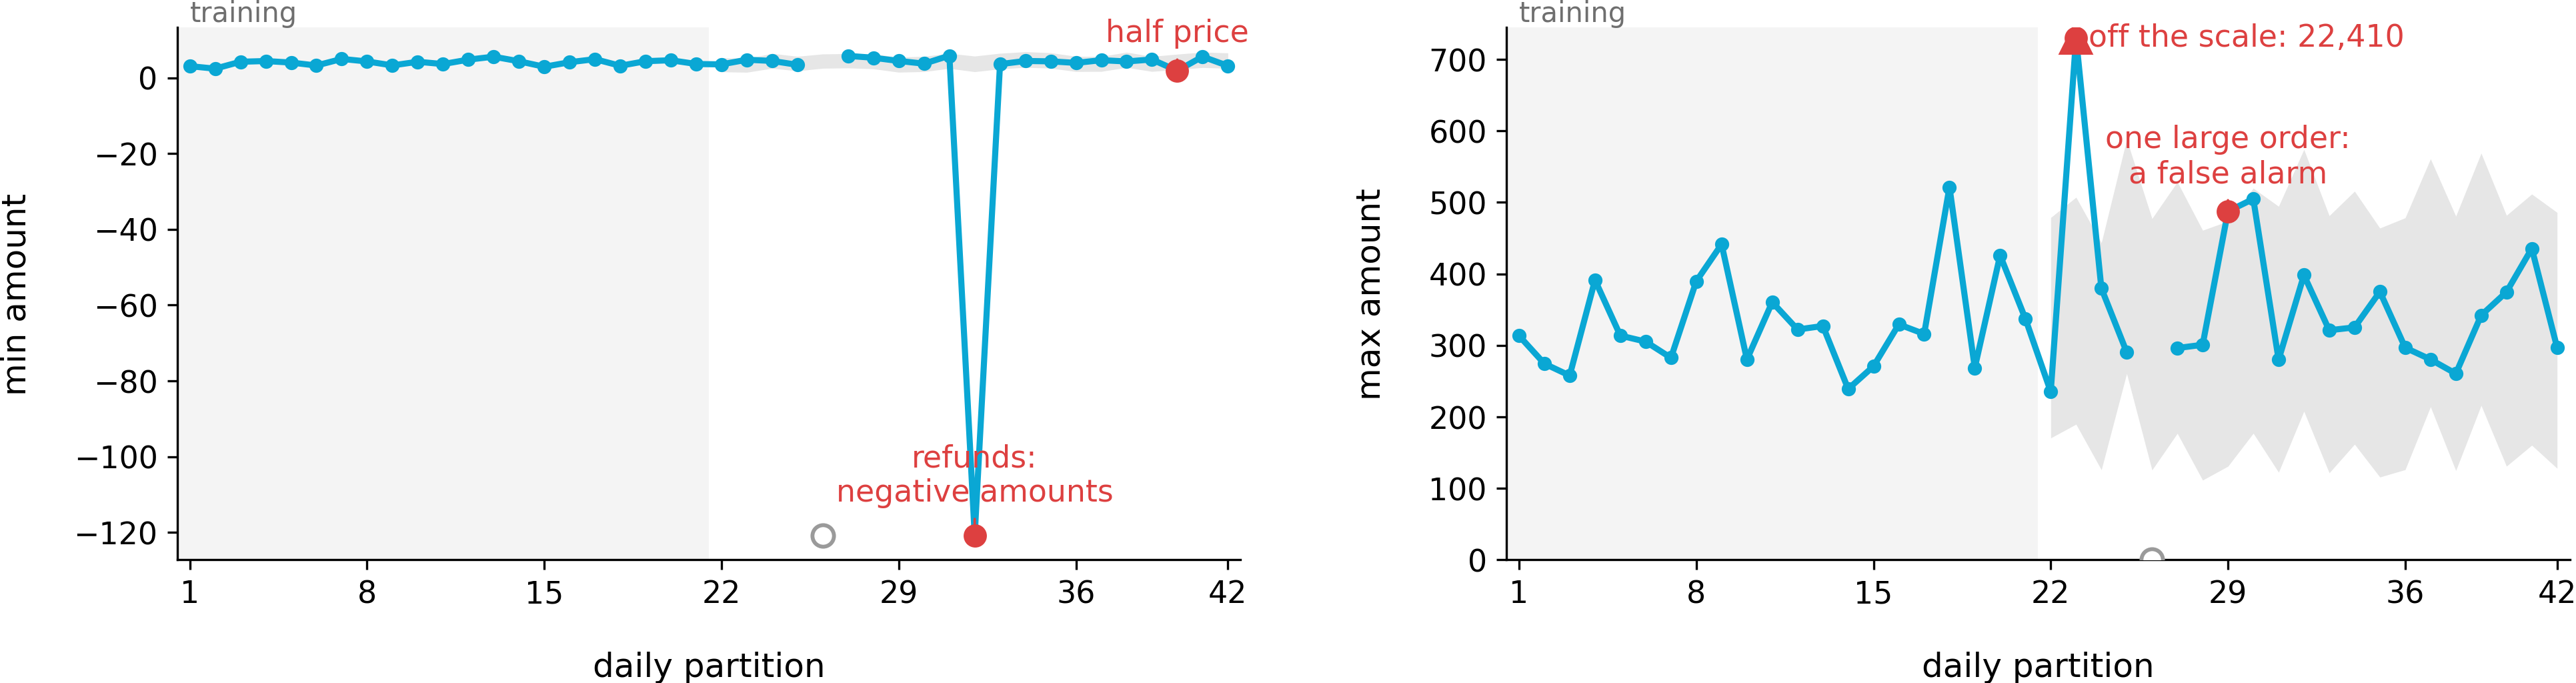
\includegraphics[width=\textwidth]{figures/Observability_min_max.png}
\end{center}

\textbf{Figure. Min and Max.} Daily order amounts. \underline{Left:} refunds on day $32$ produce a minimum of $-121$; discounts on day $40$ lower the minimum to $1.86$. \underline{Right:} amounts stored in cents on day $23$ raise the maximum to $22{,}410$, above the scale. Day $29$ also triggers an alert, but its $487$ order is valid.

\textbf{When to use it?}

Use fixed limits for known requirements, such as non-negative quantities. Use historical ranges when you want to spot unusual extremes, allowing for legitimate large or small values. Min and Max show the extremes, not how many rows are affected; count invalid rows separately if that matters.

% ---------- Quartiles ----------
\clearpage
\thispagestyle{observabilitystyle}
\section{Quartiles}\label{sec:quartiles}
\subsection{Q1, Median, Q3}

Quartiles mark three positions in a column's sorted values: one-quarter of the way through, halfway through, and three-quarters of the way through. These are Q1, the median and Q3. They help show where most values lie without being dominated by a few extremes.

% equation
\begin{center}
    \tikz{
        \node[inner sep=2pt, font=\Large] (a) {
            {
                $\displaystyle
                Q_{{\color{nmlyellow}p}}(t) = \inf \big\{\, x : {\color{nmlcyan}F_t}(x) \geq {\color{nmlyellow}p} \,\big\}, \qquad p \in \{0.25, 0.5, 0.75\}
                $
            }
        };
        \draw[overlay,-latex,nmlcyan, semithick] ($(a.south)+(-1.76,0.15)$) to node[pos=1, below] {share of values at or below $x$} +(0.00,-0.30);
        \draw[overlay,-latex,nmlyellow, semithick] ($(a.south)+(-0.21,0.13)$) to[bend right=15] node[pos=1, right] {the quantile level} +(1.00,-0.33);
    }
\end{center}

The function $F_t(x)$ gives the share of values at or below $x$, ignoring nulls. For Q1, the formula finds where that share first reaches $25\%$; the median and Q3 use $50\%$ and $75\%$. Software may estimate positions between observed values; these figures use linear interpolation.

\begin{center}
    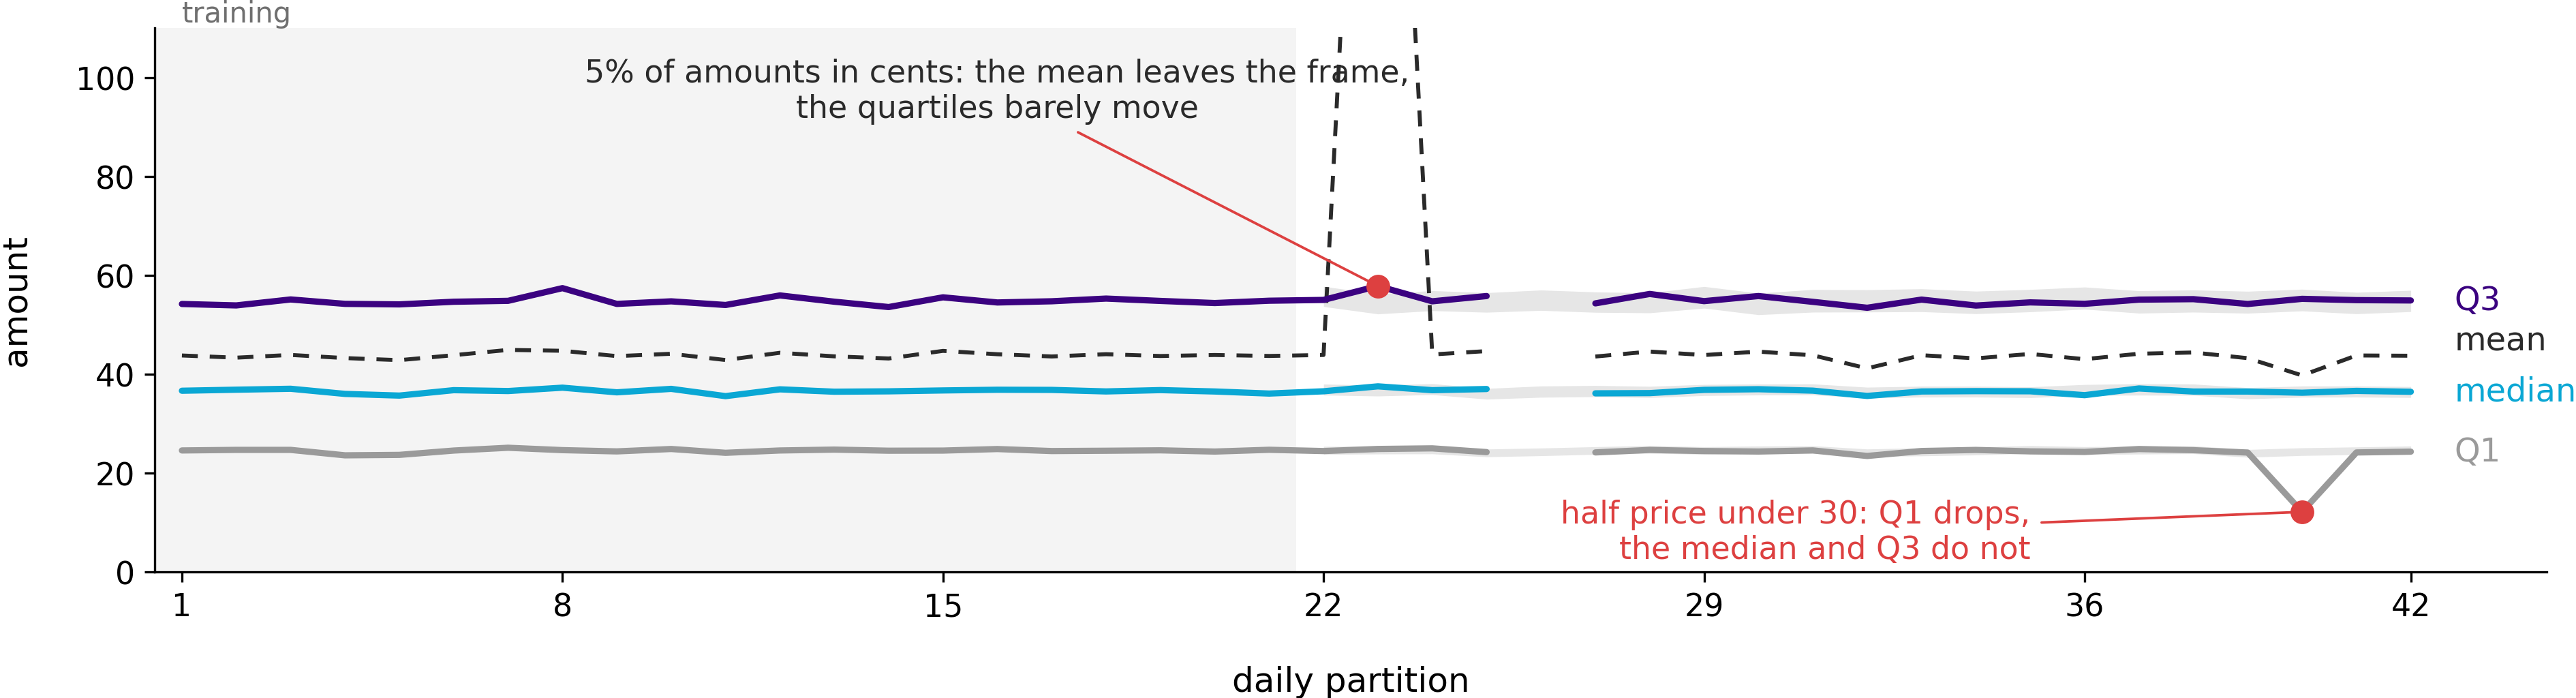
\includegraphics[width=\textwidth]{figures/Observability_quartiles.png}
\end{center}

\textbf{Figure. Quartiles.} Daily order-amount quartiles, with the mean dashed. On day $23$, about $5\%$ of amounts arrive in cents. The mean rises above the scale; Q3 rises much less but is still flagged. On day $40$, prices below $30$ are halved. Q1 drops from about $25$ to $12$; that day's median and Q3 are unaffected.

\textbf{When to use it?}

Use quartiles to track typical values and spread when a few large or small values make the mean hard to interpret. The gap between Q1 and Q3 shows the spread of the middle half of the data. Check Min and Max too if extreme values matter.

% ---------- Text Length ----------
\clearpage
\thispagestyle{observabilitystyle}
\section{Text Length}\label{sec:text-length}
\subsection{Format}

Text length counts the characters in a value. Tracking the average, shortest and longest lengths can reveal cut-off text, missing prefixes or changes in code format. Nulls are excluded, but an empty string has length zero.

% equation
\begin{center}
    \tikz{
        \node[inner sep=2pt, font=\Large] (a) {
            {
                $\displaystyle
                \overline{\ell}_t = \frac{1}{{\color{nmlred}n_t}} \sum_{r \in P_t} {\color{nmlcyan}\text{len}}\big(s(r)\big)
                $
            }
        };
        \path[room for labels] ([yshift=0.30cm]a.north) ([yshift=-0.00cm]a.south);
        \draw[overlay,-latex,nmlred, semithick] ($(a.south)+(-0.99,0.33)$) to[bend left=15] node[pos=1, left] {non-null strings} +(-1.00,-0.30);
        \draw[overlay,-latex,nmlcyan, semithick] ($(a.north)+(0.56,-0.34)$) to[bend right=15] node[pos=1, left] {characters in the string} +(-1.00,0.62);
    }
\end{center}

The formula adds the lengths of the non-null strings and divides by their count $n_t$. For lengths $[4,4,7]$, the average is $5$. Count characters rather than bytes: some characters occupy more than one byte.

\begin{center}
    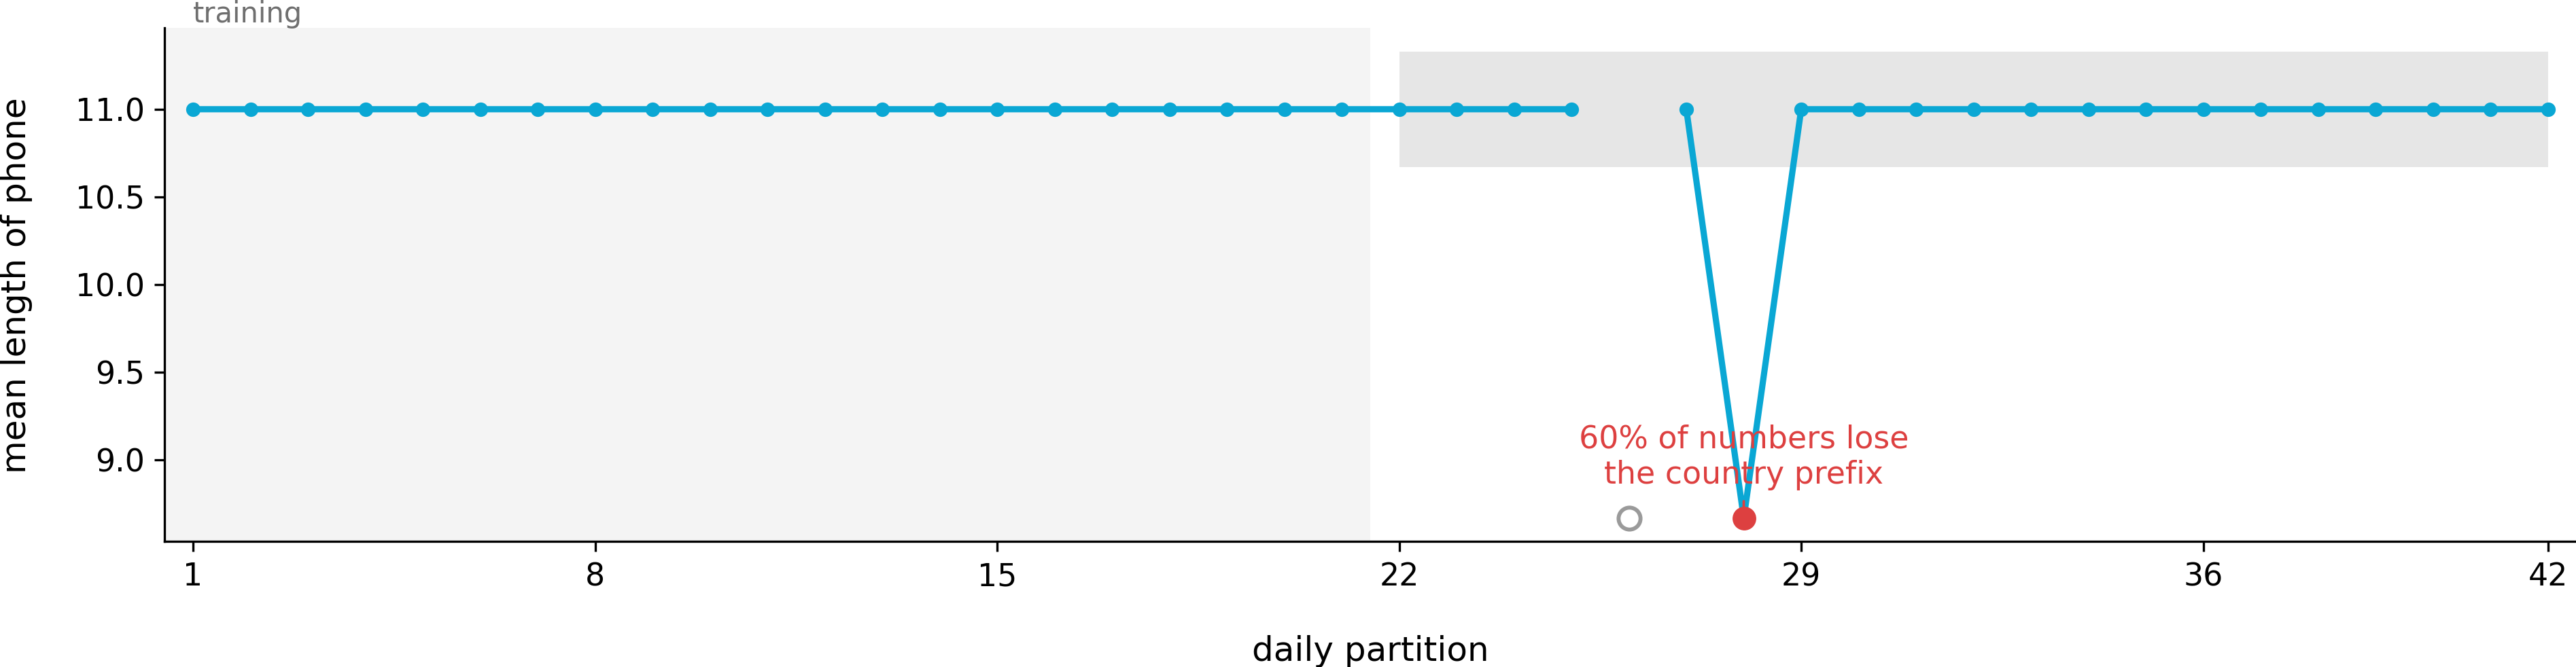
\includegraphics[width=\textwidth]{figures/Observability_text_length.png}
\end{center}

\textbf{Figure. Text Length.} Daily average length of phone values. They normally contain eleven characters, including punctuation. On day $28$, about $60\%$ arrive as seven-character values, reducing the average to $8.7$. The values are still text and none is null, so type and missing-value checks would not catch the change.

\textbf{When to use it?}

Use it on fields with a predictable format, such as product codes and phone numbers. Length alone cannot tell you whether the content is correct: two different values can have the same length. For free text, allow for normal variation before interpreting a change as an error.
